% ID: SEL-D0011-BB-E03
% ESTADO: validada. S012; tres pasadas del mismo autor, sin segundo revisor.
\textbf{a) Continuidad y derivabilidad.}\par\nopagebreak[4]
El dominio es $[-2,2]$. Las ramas polinómicas son continuas y derivables en sus interiores. En $0$,
\[
\lim_{x\to0^-}(x+1)^2=1=\lim_{x\to0^+}(x-1)^2=f(0).
\]
Es continua en todo el dominio, unilateralmente en sus extremos. Las derivadas laterales en $0$ son $2$ y $-2$: no es derivable en $0$. Para los restantes puntos interiores,
\[
f'(x)=\begin{cases}2(x+1)&-2<x<0,\\2(x-1)&0<x<2.\end{cases}
\]
En los extremos del dominio sólo cabe hablar de la correspondiente derivada unilateral.

\textbf{b) Extremos.}\par\nopagebreak[4]
De los signos de las derivadas se obtiene que decrece en $[-2,-1]$, crece en $[-1,0]$, decrece en $[0,1]$ y crece en $[1,2]$.
\[
\begin{array}{c|rrrrr}
x&-2&-1&0&1&2\\\hline
f(x)&1&0&1&0&1
\end{array}
\]
Los mínimos relativos y absolutos son \boxed{f(-1)=f(1)=0}. En $0$ hay un máximo relativo interior pese a no existir derivada. El máximo absoluto es \boxed{1}, alcanzado en \boxed{x=-2,\ 0,\ 2}. Los extremos del dominio son también máximos locales si se adopta la convención unilateral relativa al dominio.

\textbf{c) Recinto y área.}\par\nopagebreak[4]
Entre $-1$ y $1$ ambas ramas son no negativas, así que área e integral coinciden. La figura sombrea sólo el recinto pedido.
\begin{center}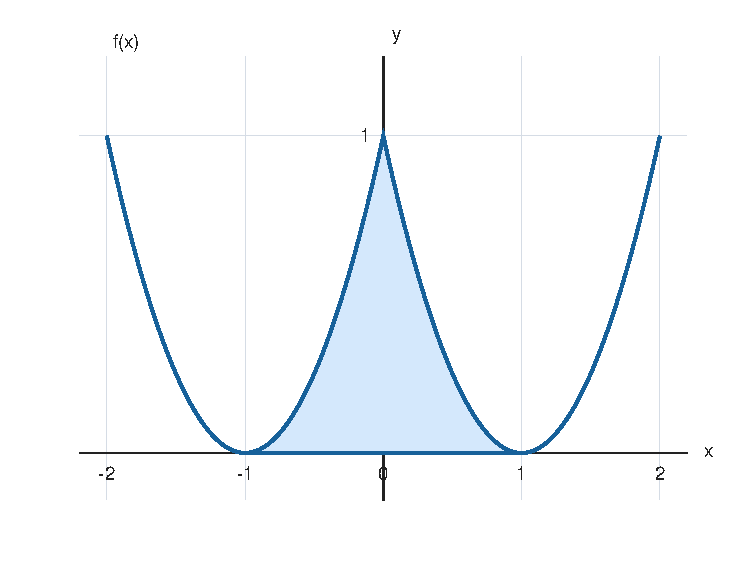
\includegraphics[width=0.58\linewidth]{recursos/figuras/s012-area.pdf}\end{center}
\[
\begin{aligned}
\mathcal A&=\int_{-1}^0(x+1)^2\,dx+\int_0^1(x-1)^2\,dx\\
&=\left[\frac{(x+1)^3}{3}\right]_{-1}^0
+\left[\frac{(x-1)^3}{3}\right]_0^1
=\frac13+\frac13=\boxed{\frac23\text{ unidades cuadradas}.}
\end{aligned}
\]
También se comprueba por simetría: el área es dos veces la de cualquiera de sus mitades.
